\documentclass[dvipdfmx]{jarticle}
\usepackage{tikz}
\usetikzlibrary{automata,calc,shapes}
\pagestyle{empty}
\begin{document}
\begin{flushright}
  \verb|2025/10/17|
\end{flushright}
\begin{center}
  {\bf\Large コンパイラ第1回演習課題(解答例)}
\end{center}

\vspace*{2cm}

\begin{enumerate}
  \item
        \begin{enumerate}
          \item $\{V_1,V_5,V_7\}$ および $\{V_2,V_5,V_7\}$

                考察：独立集合は補グラフにおけるクリークである．補グラフはノード数について多項式時間で生成できる．
                クリークを求める計算量はNP完全問題なので，独立集合を求めるのは難しい問題である．（７章における
                レジスタ割当において用られる．）

          \item 弦グラフの条件を満たす．\\
                完全消去順序は以下の４８通り（このうち一つがあればOK）
                \begin{center}
                  \begin{tabular}{llll}
                    2135467 & 2135476 & 2135647 & 2135674 \\
                    2135746 & 2135764 & 2137456 & 2137465 \\
                    2137546 & 2137564 & 2137645 & 2137654 \\
                    2173456 & 2173465 & 2173546 & 2173564 \\
                    2173645 & 2173654 & 2176345 & 2176354 \\
                    2176435 & 2176453 & 2176534 & 2176543 \\
                    2713456 & 2713465 & 2713546 & 2713564 \\
                    2713645 & 2713654 & 2716345 & 2716354 \\
                    2716435 & 2716453 & 2716534 & 2716543 \\
                    2761345 & 2761354 & 2761435 & 2761453 \\
                    2761534 & 2761543 & 2765134 & 2765143 \\
                    2765314 & 2765341 & 2765413 & 2765431 \\[1ex]
                    7213456 & 7213465 & 7213546 & 7213564 \\
                    7213645 & 7213654 & 7216345 & 7216354 \\
                    7216435 & 7216453 & 7216534 & 7216543 \\
                    7261345 & 7261354 & 7261435 & 7261453 \\
                    7261534 & 7261543 & 7265134 & 7265143 \\
                    7265314 & 7265341 & 7265413 & 7265431 \\
                    7621345 & 7621354 & 7621435 & 7621453 \\
                    7621534 & 7621543 & 7625134 & 7625143 \\
                    7625314 & 7625341 & 7625413 & 7625431 \\
                    7652134 & 7652143 & 7652314 & 7652341 \\
                    7652413 & 7652431 & 7654123 & 7654132 \\
                    7654213 & 7654231 & 7654312 & 7654321 \\
                  \end{tabular}
                \end{center}

        \end{enumerate}
  \item\ \\
        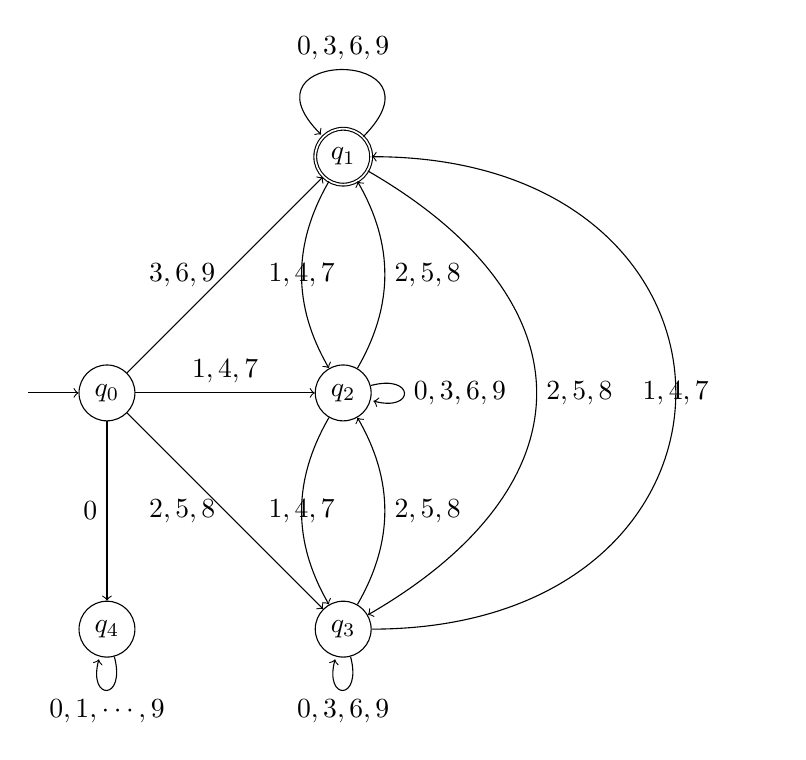
\begin{tikzpicture}
          \node[draw,circle] (Q0) at (0,3) {$q_0$};
          \node[draw,circle,double] (Q1) at (3,6) {$q_1$};
          \node[draw,circle] (Q2) at (3,3) {$q_2$};
          \node[draw,circle] (Q3) at (3,0) {$q_3$};
          \node[draw,circle] (Q4) at (0,0) {$q_4$};
          \path[->] ($(Q0)+(-1,0)$) edge (Q0);
          \path[->] (Q0) edge [left] node {$3,6,9$} (Q1);
          \path[->] (Q0) edge [above] node {$1,4,7$} (Q2);
          \path[->] (Q0) edge [left] node {$2,5,8$} (Q3);
          \path[->] (Q1) [bend right] edge  node {$1,4,7$} (Q2);
          \path[->] (Q2) [bend right] edge [right] node {$2,5,8$} (Q1);
          \path[->] (Q2) [bend right] edge node {$1,4,7$} (Q3);
          \path[->] (Q3) [bend right] edge [right] node {$2,5,8$} (Q2);
          \path[->] (Q1) [loop] edge [above] node {$0,3,6,9$} (Q1);
          \path[->] (Q3) [loop below] edge [below] node {$0,3,6,9$} (Q3);
          \path[->] (Q2) [loop right] edge [right] node {$0,3,6,9$} (Q2);
          \path[->] (Q1) [out=330,in=30,looseness=1.5] edge [right] node {$2,5,8$} (Q3);
          \path[->] (Q3) [out=0,in=0,looseness=2.2] edge node {$1,4,7$} (Q1);
          \path[->] (Q0) edge [left] node {$0$} (Q4);
          \path[->] (Q4) [loop below] edge [below] node {$0,1,\cdots,9$} (Q4);
        \end{tikzpicture}
\end{enumerate}
\end{document}
